\chapter{Definition of the Project}

	\section{Motivation}
		The project motivation is the natural continuation of a previous project performed at ICAM University. This project was part of the assembly line of a car manufacturing process and its objective was to pick some specific plastic pieces and place them into the product. To achieve this, the system used opencv image processing, so it was recognising a specific shape given apriori.
		
		This project was totally functional and the robot could perform the task with a high successful rate. However, the lack of generalization of the system makes it hard to introduce changes as using it for another part of the assembly line. Each time that this happened someone would have to introduce the shape of the pieces to the system and to calibrate the camera to the new environment. 
		
		The motivation of the project is to create from scratch a new solution for performing the picking of the pieces. This time, the project will not be sponsored by any company, so there will be less resources to use.
		
		With this new approach, the idea is to use all the knowledge of previous documented projects on Artificial Intelligence in the industry and make a little contribution to the huge advance of industry 4.0. In fact, the idea is to make the project completely replicable so that anyone could use this project as a starting point for new applications.

	\section{Objectives}

		The objectives of the project are five and are listed and explained below:
		
		\begin{itemize}
			\item[\textendash]Implement a bin picking simple solution. A basic one, without Artificial Intelligence.
			\item[\textendash]Improve the performance using RL and Image Recognition.
			\item[\textendash]Study the usage of new technologies to add information to the system. 
			\item[\textendash]Analyse the results and test new solutions to improve them. 
			\item[\textendash]Add value to the scientific community making the solution available if the previous objectives are reached.
		\end{itemize}
	
	\section{Methodology}
		This project will be performed using an agile methodology, which is one of the simplest and effective processes to turn a vision for a business need into software solutions. Agile is a term used to describe software development approaches that employ continual planning, learning, improvement, team collaboration, evolutionary development, and early delivery. It encourages flexible responses to change \cite{noauthor_agile_nodate}.
		
		In the case of this project, the team is just formed by two workers and a project manager. This make necessary to make some changes to the typical agile methodology. For example, daily meetings are substituted by constant communication between both workers and weekly meetings with the project director. With this approach, all the members of the project are updated about how it is going and have clear objectives.
		
		Likewise, the methodology of this project is based in three fundamental principles as it is shown in \autoref{fig:methodology}. The first two principles are highly related, as the project is iterative because it is experimental. That means that the way of working is perform little sprints with new functionalities, test them (experimental) and, depending on the results, define the new sprint, execute it and test again (iterative). Besides, the project is also incremental because the idea is starting implementing the simplest possible solution and keep adding new improvements to it in a iterative loop until the optimal configuration is reached.
		
		\begin{figure}
			\centering
			
\includegraphics[width=0.85\linewidth]{Images/methodology}
			\caption[Methodology]{Methodology}
			\label{fig:methodology}
		\end{figure}
		
	
	\section{Planning and budget}
	
			Regarding the planning, there are some really important functionalities that have been defined since the beginning of the project, as they are needed. These functionalities are split in three different groups: Hardware implementation, Artificial Intelligence Implementation and Robot controller implementation. The tasks related to these three groups are shown in \autoref{fig:planning1}, \autoref{fig:planning2} and \autoref{fig:planning3}. 
		
		\begin{figure}
			\centering
			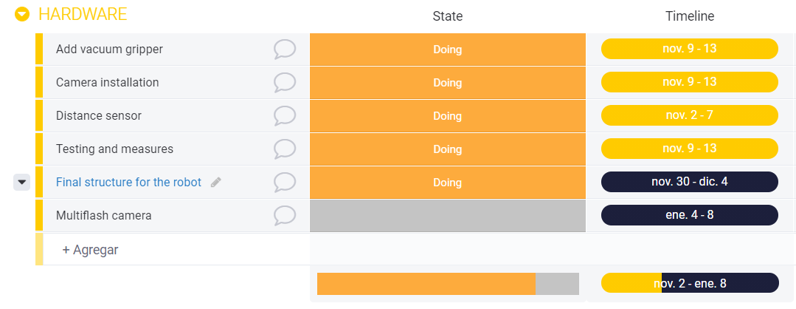
\includegraphics[width=0.85\linewidth]{Images/planning1}
			\caption[Chronograph HW]{Chronograph of the Hardward implementation}
			\label{fig:planning1}
		\end{figure}
	
		\begin{figure}
			\centering
			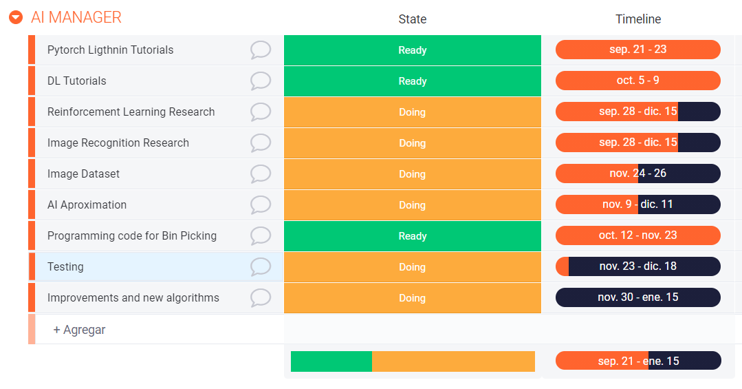
\includegraphics[width=0.85\linewidth]{Images/planning2}
			\caption[Chronograph HW]{Chronograph of the Hardward implementation}
			\label{fig:planning2}
		\end{figure}
		
		\begin{figure}
			\centering
			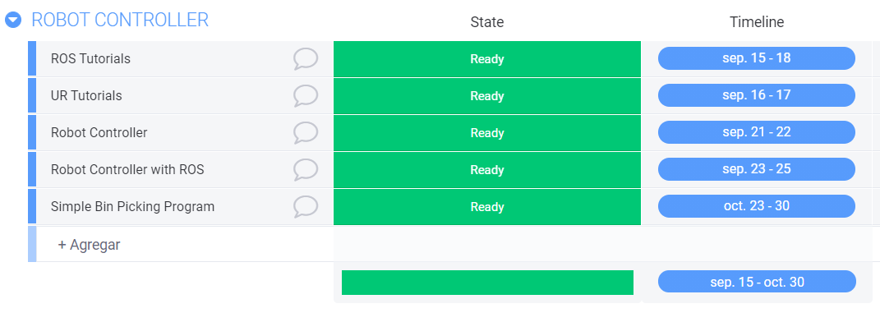
\includegraphics[width=0.85\linewidth]{Images/planning3}
			\caption[Planing Robot Controller]{Planning of the Robot Controller implementation}
			\label{fig:planning3}
		\end{figure}
		
		\subsection{Budget}
			The budget of the project was really limited because it was not sponsored by any company. The cost was mainly due to hardware acquisition. For example, the gripper was design and built by us in order to save thousands of euros.
			
			In the following table we can see the detailed budget of all the project:
			
			\begin{center}
				\begin{tabular}{ccc}
					\toprule 
					ITEM & QUANTITY & PRICE  \\ 
					\midrule
					Nvidia Geoforce GTX & 2 & 395,88 \\
					\rowcolor{black!20}Vacuum Gripper & 1 & 53,50 \\
					Raspberry Pi4 & 1 & 59,05 \\
					\rowcolor{black!20}Electronic Parts & (Sensors, transistors..) & 30 \\
					Arduino  & 1 & 22,64 \\
					\rowcolor{black!20}HDMI->VGA & 2 & 63,31 \\
					QWERTY keyboards & 2 & 36,85 \\
					\bottomrule
					& Total & 661,23 \\
				\end{tabular}
				\captionof{table}{Project's Budget}
				\label{tab:budget}
			\end{center}
			